\chapter{Introduction}

\epigraph{\textit{Light thinks it travels faster than anything but it is wrong. No matter how fast light travels, it finds the darkness has always got there first, and is waiting for it.}}{Terry Pratchett -- \textit{Reaper Man}}

\vspace{1cm}
\par\noindent In this thesis, I discuss the physics of matter in close proximity to neutron stars\index{Neutron star} and black holes\index{Black hole}.  These astrophysical entities, collectively referred to as `compact objects'\index{Compact object}, are the densest objects known to exist in our universe, and are formed in the death throes of massive stars.
\par When a star with a mass between $\sim8$--10\,$M_\odot$\footnote{1\,$M_\odot\approx2\times10^{30}$\,kg, or one times the mass of our Sun.} (e.g. \citealp{Bildsten_NS}) runs out of nuclear fuel in its core, it is no longer able to support its own weight and collapses inwards.  This collapse generates a shockwave which disrupts the star, resulting in most of the star being ejected in an event known as a supernova\index{Supernova}.  The core of the star survives this disruption and continues collapsing.  The core of a massive star is supported by electron degeneracy pressure; a pressure caused by the fact that no two fermions can occupy the same quantum state \citep{Pauli_Exclusion}.  However, during the collapse of the core in a supernova, even electron degeneracy pressure cannot support the star; when the core has a mass greater than 1.4\,M$_\odot$ (the Chandrasekhar Limit, \citealp{Chandrasekhar_Mass}), electrons merge with protons via inverse $\beta$-decay, forming an object supported mostly by neutron degeneracy pressure.  The resulting `neutron star'\index{Neutron star} is an extremely dense object, with a mass of several M$_\odot$ compressed into a sphere with a radius of $\sim20$\,km.  Additionally as the core collapses, it spins up to conserve angular momentum until it is rotating at a rate of $\sim100$\,Hz.  The extreme gravitational field in the proximity of such a strong object results in a region of space which is strongly affected by the effects predicted by general relativity \citep{Einstein_GR}\index{General relativity}.  The extremely rapid rotation of neutron stars, and the associated high-velocity electron and proton populations present in their cores (e.g. \citealp{Alpar_Impure}), can result in magnetic fields as strong as $\sim10^{15}$\,G\footnote{1 Gauss, or 1\,G, is equal to 10$^{-4}$ Tesla, where Tesla is the SI-derived unit of magnetic field strength.} \citep{Woltjer_NSB,Gold_Pulsar,Kaspi_Magnetar}.  For a collapsing star with a mass of greater than $\sim10$\,M$\odot$, the end product is even more extreme.  The core of such a star can become so dense during a supernova that even neutron degeneracy pressure cannot support it, and instead it collapses into a black hole\index{Black hole}; a region of space with such a strong gravitational field that no information can escape it.
\par Unfortunately, compact objects\index{Compact object} are inherently faint objects.  In fact, an isolated black hole\index{Black hole} is theoretically only visible via the effects its gravitational well has on the light from stars located behind it.  As such, observational research into these objects tends to focus one of two types of system: Active Galactic Nuclei (AGN) and X-Ray Binaries (XRBs)\index{X-ray binary}.  In both of these types of system a compact object gravitationally attracts matter from its surrounding enviroment, a process known as `accretion'\index{Accretion}.  The act of matter falling into such a steep gravitational well causes large amounts of energy to be released; as such, these systems shine brightly in high-energy regions of the electromagnetic spectrum such as the X-rays and $\gamma$-rays.
\par AGN\index{Active galactic nucleus} contain supermassive black holes\index{Black hole}\index{Black hole!Supermassive black hole} with masses upwards of $\sim10^6$\,$M_\odot$ (e.g. \citealp{Miyoshi_SMBH}).  These black holes are believed to be present at the centre of all large galaxies but many, such as Sagittarius A$^\star$ in our Milky Way, are currently dormant and not significantly accreting\index{Accretion} \citep{LyndenBell_Quasar,Schodel_SagA}.  AGN are the brightest persistent sources of electromagnetic radiation in the universe, and they launch powerful `jets' of matter out to distances of many kiloparsec (kpc\footnote{$1$\,kpc$ =1000$\,parsec $\approx3\times10^{19}$\,m.  A parsec is the distance of an object that shows a parallax of 1'' (1 arcsecond, or $\frac{1}{3600}$ of a degree) against background objects when viewed from opposing points along the orbit of the Earth.}).  AGN have been implicated as having an important role in the development of their host galaxies via a process known as AGN feedback, in which mechanical and electromagnetic power from the AGN is `fed back' into its host galaxy and influences its evolution.
\par Active Galactic Nuclei are very distant systems.  Because of the large size of these objects, they also only evolve over timescales of thousands of years.  These facts make studying some of the properties of matter in a relativistic regime difficult to determine by only observing AGN.  Thankfully, there exists a population of bright, accreting\index{Accretion} compact objects\index{Compact object} much closer to home: XRBs\index{X-ray binary}.

\section{Anatomy of an X-Ray Binary}

\index{LMXB|see {X-ray binary, Low mass}}
\index{IMXB|see {X-ray binary, Intermediate mass}}
\index{HMXB|see {X-ray binary, High mass}}
\index{XRB|see {X-ray binary}}
\par In this thesis, I will be focusing on XRBs\index{X-ray binary}.  These systems are physically much smaller than AGN\index{Active galactic nucleus}\index{AGN|see {Active galactic nucleus}}, with compact objects\index{Compact object} no more massive than $\sim20\,M_\odot$, but in many ways they can be more extreme.  The gravitational tidal forces close to the compact object are greater than in AGN and, due to their small size, XRBs can evolve rapidly over timescales of seconds or less.
\par An XRB is a system containing a compact object\index{Compact object}\footnote{A black hole\index{Black hole} or a neutron star\index{Neutron star}.  Similar systems with a white dwarf\index{White dwarf} as their compact object are referred to as Cataclysmic Variables (CVs)\index{Cataclysmic variable}\index{CV|see {Cataclysmic variable}}.} and a main sequence or giant companion star\index{Companion star}\index{Stellar companion|see {Companion star}}.  By various processes, matter is lost from the companion star and transferred onto the compact object.  In order to conserve angular momentum\index{Angular momentum}, matter cannot simply fall onto the compact object; instead this matter spirals inwards, forming a large disk of material.  Frictional forces in the inner portions heat this `accretion disk'\index{Accretion disk} to extreme temperatures $\gtrsim1$\,keV\footnote{1\,keV$=1000$\,eV$=1.6\times10^{-16}$\,J .  1\,eV (electron-Volt) is the amount of energy an electron gains by crossing a potential difference of 1\,V.  Although this is a unit of energy, it is often used in high-energy physics to denote temperature by describing the energy at which the emission of a black body at that temperature is peaked.  1\,keV corresponds to a temperature of $\sim1.16\times10^7$\,K}.  In some XRBs, so much X-ray radiation is released in this process that the pressure from photons\index{Radiation pressure}, which is negligible but non-zero under standard conditions, becomes important to describe the equation of state of the disk.

\subsection{Types of X-Ray Binaries: High and Low-Mass}

\par XRBs are divided into two broad categories depending on the mass of the companion star\index{Companion star} and, in turn, the predominant mechanism responsible from transferring matter from the star to the compact object\index{Compact object}.  High Mass X-ray Binaries (HMXBs)\index{X-ray binary!High mass} have a companion star with a mass $\gtrsim10\,M_\odot$.  High mass stars tend to be unstable, and these objects can eject large quantities of matter in a stellar wind.  In a HMXB, part of this stellar wind is gravitationally captured by the compact object and feeds the accreting\index{Accretion} compact object.
\par Low Mass\index{X-ray binary!Low mass} and Intermediate Mass\index{X-ray binary!Intermediate mass} X-Ray Binaries (LMXBs/IMXBs), systems in which the mass $M$ of the companion star is $M\lesssim1\,M_\odot$ and 1M$_\odot\gtrsim M\lesssim10$M$_\odot$ repsectively, accrete\index{Accretion} matter in a different way.  Each object in an astrophysical binary system has a Roche Lobe\index{Roche lobe}: a teardrop-shaped region of space in which it is gravitationally dominant.  Inside the Roche Lobe matter is gravitationally bound to the central star, while matter outside of the lobe is free to escape.
\par Under some circumstances, it is possible for a star to become larger than its Roche lobe.  This can happen in two main ways:
\begin{enumerate}
\item The radius of the binary orbit decreases, shrinking the Roche Lobe of each object.
\item The radius of the star increases.  This can happen, for example, when the star evolves from the Main Sequence onto the Giant branch.
\end{enumerate}
In either scenario, a portion of the star ends up within the Roche lobe\index{Roche lobe} of the compact object\index{Compact object}.  This matter is free to spiral onto the compact object, forming the accretion disk\index{Accretion disk} (e.g. \citealp{Lewin_SSRev}).

\subsection{Components of a Low Mass X-Ray Binary}

\par As well as the accretion disk\index{Accretion disk}, there are several additional features present in a typical X-Ray Binary; I show a schematic of an LMXB in Figure \ref{fig:xrbcartoon}.   Radio observations of nearby XRBs (e.g. \citealp{Mirabel_Microquasar,Geldzahler_Jet}) have shown that these systems can show axial jets\index{Jet} of material similar to those seen in AGN; in Figure \ref{fig:jet} I show a radio image from \citet{Fender_1915} showing a jet being launched from the LMXB GRS 1915+105\index{GRS 1915+105}. These jets can eject matter at velocities approaching the speed of light $c$ (e.g. \citealp{Mirabel_Microquasar}).

\begin{figure}
    \includegraphics[width=\columnwidth, trim = 0mm 0mm 0mm 0mm]{images/xrbcartoon.eps}
    \captionsetup{singlelinecheck=off}
    \caption[A cartoon illustrating the basic geometry of a simple X-ray binary.]{A cartoon illustrating the basic geometry of a simple low mass X-ray binary\index{X-ray binary!Low mass}.  Not shown is the non-thermal corona\index{Corona} of material which can be inferred from spectroscopy, as the geometry of this feature is disputed.  Diagram not to scale.}
   \label{fig:xrbcartoon}
\end{figure}

\begin{figure}
   \centering
    \includegraphics[width=0.6\columnwidth, trim = 0.1mm 0.2mm 0.1mm 0.2mm, clip]{images/contour.png}
    \captionsetup{singlelinecheck=off}
    \caption[A series of 5\,GHz radio images from \citet{Fender_1915} showing a jet being launched from the LMXB GRS 1915+105.]{A series of 5\,GHz radio images, advancing in time from top to bottom, showing a two-lobed jet of material flowing away from GRS 1915+105\index{GRS 1915+105} (at 0 milliarcseconds) at speeds approaching $c$.  Figure adapted from \citet{Fender_1915}.}
   \label{fig:jet}
\end{figure}

\par X-ray spectral studies of LMXBs find that, in addition to a black-body\footnote{The radiative power per unit frequency of a black body at temperature $T$ is given by \[F_T(\nu)=\frac{N\nu^3}{e^\frac{h\nu}{k_BT}-1}\] for some constant $N$ \citep{Planck}.  $k_B$ is the Boltzmann Constant, and $c$ is the speed of light in a vacuum.} like accretion disk\index{Accretion disk}, the systems must each contain a non-thermal `corona'\index{Corona} component.  The corona is a region of non-thermal electrons somewhere in the vicinity of the compact object\index{Compact object}, and it emits X-rays via Compton upscattering\index{Compton scattering}.  In this process, photons emitted from the disk collide with energetic electrons in the corona.  The photons, on average, gain energy from these collisions and are scattered back into space; some in the direction of observers on the Earth.  This leads to a characteristic power-law\footnote{A power-law distribution is any distribution with the functional form $f(x)=cx^k$ for some constants $c$ and $k$.} energy distribution signature at high energies, which can be seen in the spectra of LMXBs.  As I show in the simulated LMXB energy spectrum in Figure \ref{fig:toyspec}, the emission from the corona tends to dominate above energies of $\sim10$\,keV.
\par Models of the geometry of the coronal region have evolved over the years.  While the corona has been historically treated as if it was a single point fixed above the centre of the disk\index{Accretion disk} (the so-called `Lamp Post' model, e.g. \citealp{Rozanska_Lamppost}), more recent models tend to treat it either as an optically thin\footnote{An optically thin medium is defined as a medium in which an average photon interacts $<1$ times while passing through.} flow of material onto the compact object\index{Compact object} or equate it with the base of the radio jet\index{Jet} (e.g. \citealp{Skipper_CoronaGeo}).

%\begin{figure}
%   \centering
%    \includegraphics[width=0.7\columnwidth, trim = 10mm 0mm 10mm 10mm, clip]{images/toy_spec.eps}
%    \captionsetup{singlelinecheck=off}
%    \caption[A simulated, simplified spectrum of an LMXB in the high/soft state, showing the two main components visible in X-ray: the accretion disk and the corona.]{A simulated, simplified spectrum of an LMXB in the high/soft state  (see Section \ref{sec:states}), showing the two main components visible in X-ray: the accretion disk (blue) and the corona (orange).  The disk is generally modelled as a disk black body, a sum of black bodies at different temperatures corresponding to different annuli in the disk (e.g. \citealp{Mitsuda_diskbb}), while the corona is modeled as a power law.  Spectrum based on spectral fits to the LMXB MXB 1658-298, performed by \citet{Sharma_vals}.}
%   \label{fig:toyspec}
%\end{figure}

\begin{figure}
   \centering
    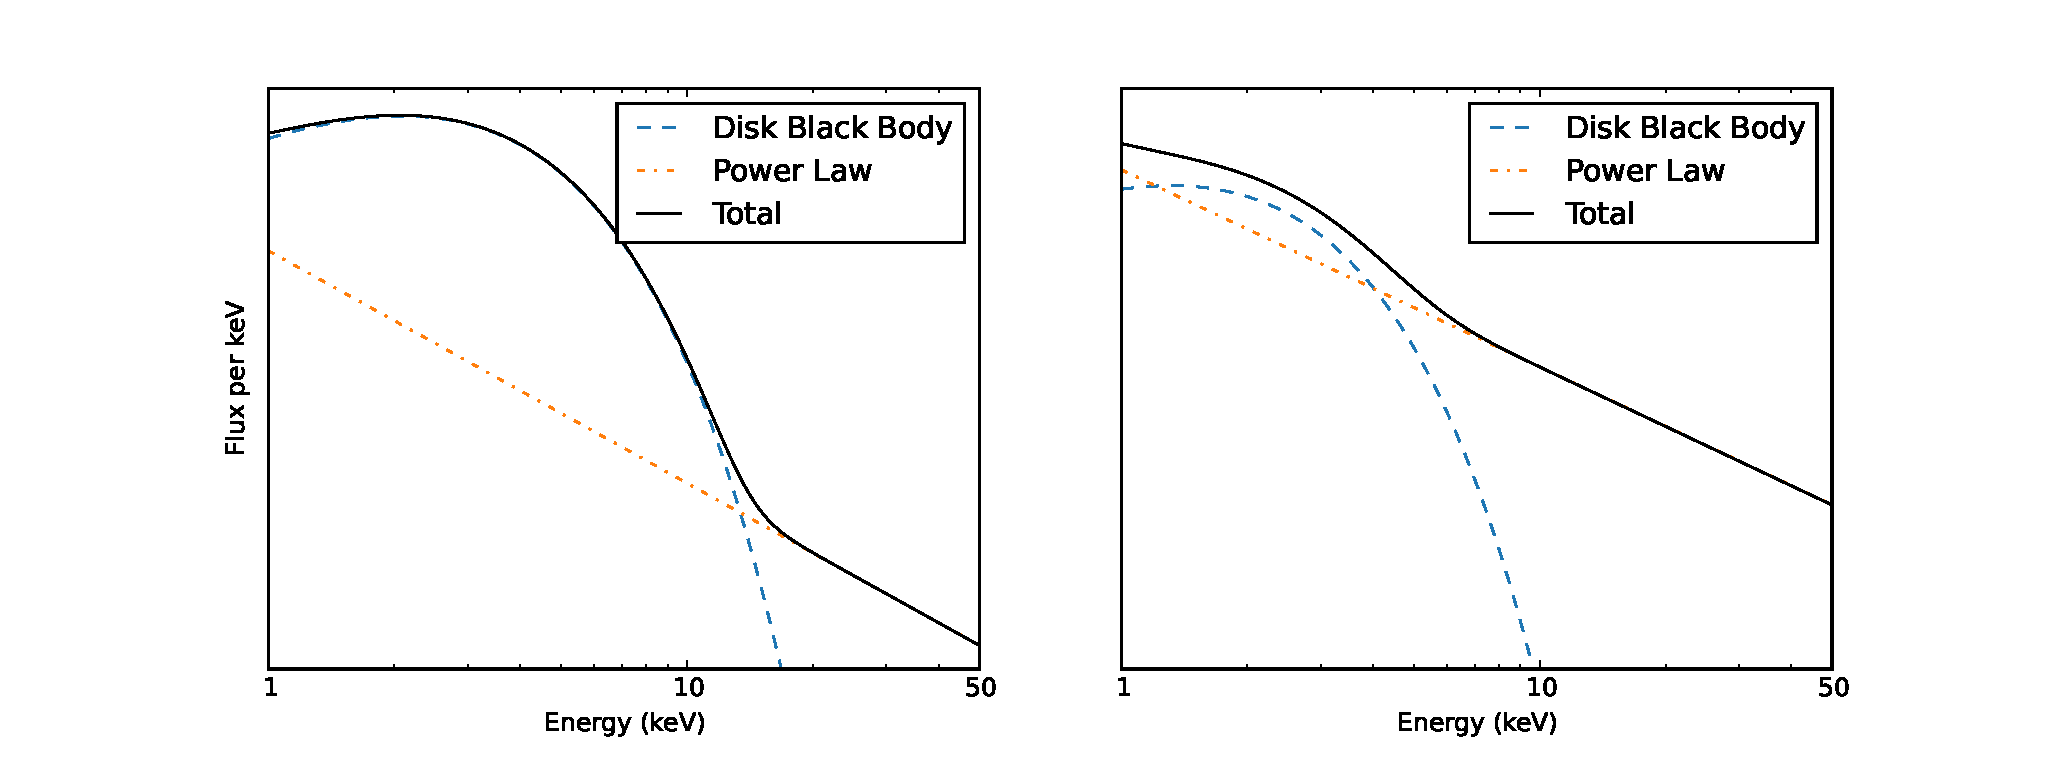
\includegraphics[width=\columnwidth, trim = 10mm 0mm 10mm 10mm, clip]{images/2toyspec.eps}
    \captionsetup{singlelinecheck=off}
    \caption[Two simulated, simplified spectra of an LMXB, showing the two main components visible in X-ray: the accretion disk and the corona.]{Two simulated, simplified spectrum of an LMXB, showing the two main components visible in X-ray: the accretion disk\index{Accretion disk} (blue) and the corona\index{Corona} (orange).  The disk is generally modelled as a disk black body, a sum of black bodies at different temperatures corresponding to different annuli in the disk (e.g. \citealp{Mitsuda_diskbb}), while the corona is modeled as a power law.  The left panel shows a typical spectrum of an LMXB in the high/soft state, while the right panel shows a typical spectrum of an LMXB in the low/hard state: see Section \ref{sec:states} for a discussion of accretion states.  These spectra are based on spectral fits to the LMXB MXB 1658-298, performed by \citet{Sharma_vals}.}
   \label{fig:toyspec}
\end{figure}

\par Another important component of an X-ray binary\index{X-ray binary} is the disk wind\index{Wind}\index{Disk wind|see {Wind}} \citep{vanParadijs_Wind}.  Due to the high temperatures and pressures in the inner part of the accretion disk\index{Accretion disk}, matter on the surface of the disk can obtain enough energy to escape the gravitational well of the compact object\index{Compact object}.  This matter is ejected from the system in large-scale, high velocity winds.  Studies of the spectral lines present in these winds have shown that they can have speeds approaching the speed of light (e.g. \citealp{Ponti_Wind,Degenaar_BPSpec}).

\subsubsection{Neutron Star X-ray Binaries}

\label{sec:NSintro}

\par The geometry of an X-ray binary is somewhat more complicated when the compact object\index{Compact object} is a neutron star\index{Neutron star}.  Unlike black holes, neutron stars are in general highly-magnetised systems, and the introduction of a large, strong magnetic field\index{Magnetic field} to an XRB has implications for the geometry of the accretion\index{Accretion} flow.  At some radius in the inner accretion disk\index{Accretion disk}, it is possible that the pressure\index{Magnetic pressure} exerted by this magnetic field becomes dominant over the gas\index{Ram pressure} and photon pressures\index{Radiation pressure}\index{Photon pressure|see {Radiation pressure}}.  At this point, ionised material becomes `frozen-in' to the magnetic field lines, and is only able to freely move along them.  Due to the extreme temperatures present in the inner portion of the accretion disk\index{Accretion disk}, the vast majority of material in this region is ionised.  This acts to disrupt the flow of material in the inner part of the accretion disk, and matter is funneled along field lines and onto the poles of the neutron star.  This causes the poles of the neutron star to become extremely hot.  As the neutron star spins, it appears to pulse as seen by an external observer due to the highly radiating magnetic poles coming in and out of view.  These objects are referred to as accreting X-ray pulsars\index{Pulsar}.
\par In addition to the effects of the magnetic field, there is another significant difference between neutron star\index{Neutron star} and black hole\index{Black hole} binaries.  Black holes are surrounded by an event horizon\index{Event horizon} from which no light can emerge, therefore there can be no direct emission from the compact object in a black hole X-ray binary.  Neutron stars on the other hand have a visible surface.  As such the surface of the neutron star itself, and any phenomena that take place there, can in principle be seen.
\par One of the most spectacular events that can occur on the surface of a neutron star\index{Neutron star} is a Type I X-ray burst \citep{Grindlay_TypeI}\index{X-ray burst!Type I}.  These occur when matter accreted\index{Accretion} onto the surface of the neutron star reaches a critical temperature and density ($\sim2.2\times10^9$\,K and $3\times10^6$\,g\,cm$^{-3}$, \citealp{Joss_TypeI}), and nuclear fusion is triggered.  This results in a flash of energy, which causes a runaway thermonuclear\index{Thermonuclear burning} explosion across most or all of the neutron star surface.  Type I bursts appear in data as a sudden increase in X-ray flux (1--2 orders of magnitude), followed by an power-law decay as the neutron star surface cools.  As Type I bursts are distinctive features which require a surface on which to occur, they are often used as a diagnostic tool to identify an unknown compact object\index{Compact object} as a neutron star.

\section{Low Mass X-Ray Binary Behaviour}

\par LMXBs\index{X-ray binary!Low mass} are not static systems, and most show variations in their luminosities over timescales of milliseconds to years.  Broadly speaking, LMXBs can be divided into persistent systems\index{Persistent source} and transient\index{Transient source} systems.  Persistent systems have always observed to be bright since their discovery, implying a high rate\index{Accretion rate} of accretion\index{Accretion} at all times.  In some objects, this bright, high-accretion rate state has persisted for $\geq20$ years (e.g. GRS 1915+105\index{GRS 1915+105}, \citealp{Deegan_1915}).
\par Transient\index{Transient source} LMXBs\index{X-ray binary!Low mass} have a somewhat more complicated life cycle.  These objects spend most of their time in a `quiescent' state\index{Quiescence}, during which they are faint in X-rays and only a relatively small amount of material is being accreted\index{Accretion}.  However these objects also undergo `outbursts'\index{Outburst}, during which their luminosity increases by many orders of magnitude for a period of days to years (e.g. \citealp{Frank_Outbursts}).  The frequency of these outbursts varies widely between sources, ranging from one every month or so to one every few decades or longer.

\label{sec:states}

\par XRB outbursts tend to follow predictable evolutionary paths, evolving through a number of different `states' as they progress.  I show some of the states associated with black hole\index{Black hole} LMXB\index{X-ray binary!Low mass} outbursts\index{Outburst} in Figure \ref{fig:Fender} on a so-called `hardness-intensity diagram'\index{Hardness-intensity diagram}\index{HID|see {Hardness-intensity diagram}}, which traces how the brightness and the spectral shape of a source evolve over time (see Section \ref{sec:hids} for more information on hardness-intensity diagrams).  At the start of a typical black hole LMXB outburst emission from the source is spectrally hard\index{Colour}\index{Hardness|see {Colour}}, i.e. dominated by higher-energy photons.  This part of the outburst is referred to as a Low/Hard State\index{Low/Hard state}\index{Hard state|see {Low/Hard state}} (bottom-right of Figure \ref{fig:Fender}), and a radio jet\index{Jet} is generally visible at this time.  The luminosity of the source gradually increases until it reaches some maximum, and then emission begins to become softer as the system heads towards the High/Soft State\index{High/Soft state}\index{Soft state|see {High/Soft state}} (top-right of Figure \ref{fig:Fender}).  During this transition, the system crosses the so-called `jet line', and the radio jet switches off.  Sources tend to spend a large portion of their outbursts in the high/soft state, appearing to meander in the hardness-intensity diagram.  This meandering may include additional crossings of the jet line, causing the radio jet to flicker on and off during this period.  The X-ray luminosity of the source then decreases, before the source returns to the hard state along a path of approximately constant luminosity.  The source then fades back into quiescence.  This typical outburst behaviour forms a distinctive `q' shape in the hardness-intensity diagram, as I show in Figure \ref{fig:Fender}, and can be thought of as the inner accretion disk\index{Accretion disk} filling with matter before draining onto the compact object\index{Compact object} or flowing out of the system in winds\index{Wind} or a jet\index{Jet} (e.g. \citealp{Fender_UniJets}).  I show typical spectra of an XRB in the low/hard\index{Low/Hard state} and high/soft\index{High/Soft state} states in Figure \ref{fig:Yamada_Spec}, taken from \citet{Yamada_Spec}.

\begin{figure}
   \centering
    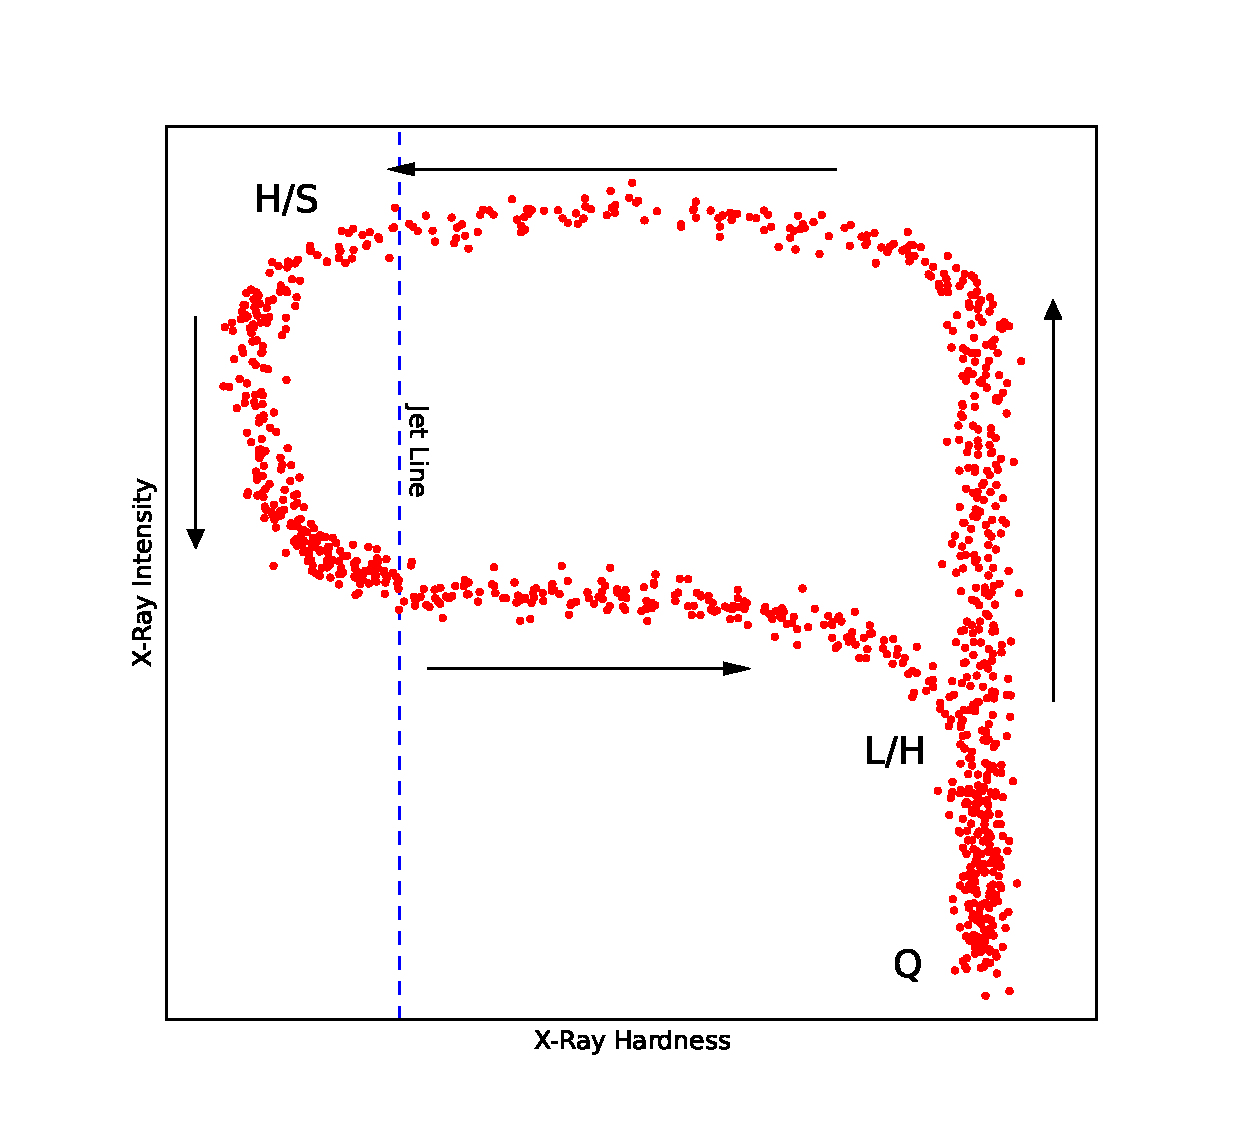
\includegraphics[width=\columnwidth, trim = 10mm 13mm 10mm 15mm, clip]{images/Fender_D.eps}
    \captionsetup{singlelinecheck=off}
    \caption[A schematic hardness-intensity diagram adapted from \citet{Fender_UniJets}, showing the evolutionary path of a typical black hole LMXB outburst.]{A schematic hardness-intensity diagram\index{Hardness-intensity diagram} adapted from \citet{Fender_UniJets}, showing the evolutionary path of a typical black hole\index{Black hole} LMXB\index{X-ray binary!Low mass} outburst\index{Outburst} and roughly indicating the positions of quiescence (Q)\index{Quiescence} and the the Low/Hard (L/H)\index{Low/Hard state} and High/Soft (H/S)\index{High/Soft state} States.  The jet line roughly demarcates the portion of the outburst in which a jet\index{Jet} is observed (right of the line) from the portion in which it is not observed (left of the line).}
   \label{fig:Fender}
\end{figure}

\begin{figure}
   \centering
    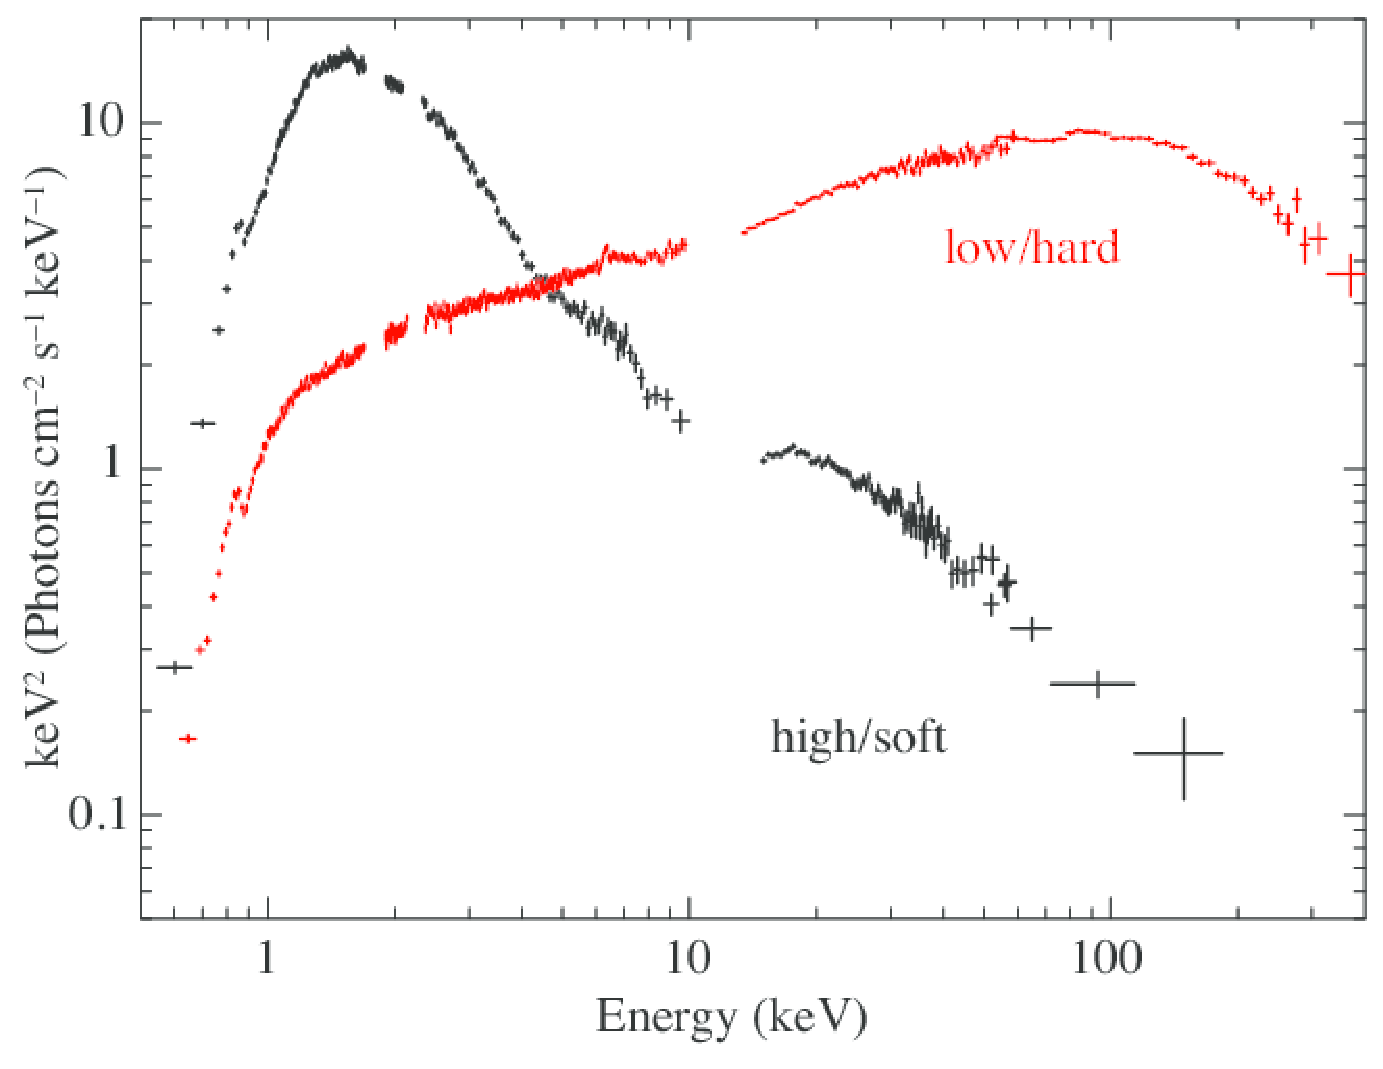
\includegraphics[width=\columnwidth, trim = 0mm 0mm 0mm 0mm, clip]{images/Yamada_Spec.eps}
    \captionsetup{singlelinecheck=off}
    \caption[Energy spectra of the black hole HMXB Cygnus X-1 in its low/hard and high/soft states, presented as typical spectra of a black hole XRB in these states.]{\textit{Suzaku}\indexsuzaku\ energy spectra of the black hole\index{Black hole} HMXB\index{X-ray binary!High mass} Cygnus X-1\index{Cyg X-1} in its low/hard\index{Low/Hard state} (black) and high/soft\index{High/Soft state} (red) states, presented as typical spectra of a black hole XRB in these states.  Figure taken from \citet{Yamada_Spec}.}
   \label{fig:Yamada_Spec}
\end{figure}

\par Neutron Star\index{Neutron star} LMXBs\index{X-ray binary!Low mass} on the other hand tend to follow one of two patterns during outburst\index{Outburst}, dividing them into so-called `Z sources'\index{Z source} and `atoll sources'\index{Atoll source} (e.g. \citealp{vanderKlis_ZAtoll}).  In Figure \ref{fig:Zatoll} I show examples of colour-colour diagrams\index{Colour-colour diagram}\index{CCD|see {Colour-colour diagram}} (which plots two different hardness ratios against each other, see Section \ref{sec:hids}) for typical Z-type and atoll-type sources.  Z sources trace out a number of `branches' during outburst, each corresponding to a period of different source behaviour.  Atoll sources on the other hand spend most of the time in the so-called `banana branch' on the colour-colour diagram, occasionally jumping over to the `island state' at larger values of hard and soft colour.  Unlike black hole LMXBs which trace out their characteristic evolutionary pattern once per outburst, Z and atoll sources trace out their evolutionary paths many times per outburst.  Z sources can complete the entire `z' over timescales of days.  Most Z sources are classified as persistent\index{Persistent source} objects, although some Z sources are transient\index{Transient source} \citep{Homan_TZ}.  On the other hand most atoll sources are transient, but some have been observed to be persistent (e.g. \citealp{Hasinger_PersAtoll}).  In addition to this, at least one source is known to change between Z- and atoll-like evolutionary patterns over time \citep{Barret_Flip}.  This complex evolution over the course of each outburst highlights the fact that accretion\index{Accretion} is not a simple process, and that understanding accretion gives us better understanding of a areas of the physics of matter in extreme environments.

\begin{figure}
   \centering
    \includegraphics[width=\columnwidth, trim = 1mm 1mm 1mm 1mm, clip]{images/Zatoll.png}
    \captionsetup{singlelinecheck=off}
    \caption[Colour-Colour diagrams from \citet{vanderKlis_ZAtoll} showing typical evolutionary paths of Atoll-type and Z-type Neutron Star LMXBs.]{Colour-colour diagrams from \citet{vanderKlis_ZAtoll}, showing evolutionary paths of typical outbursts of Atoll-type\index{Atoll source} and Z-type\index{Z source} neutron star\index{Neutron star} LMXBs\index{X-ray binary!Low mass} (GX 13+1\index{GX 13+1} and Cyg X-2\index{Cyg X-2} respectively).  On the right-hand panel, the typical `branches' of a Z-type source are marked: the High Branch (HB), Normal Branch (NB) and Flaring Branch (FB).}
   \label{fig:Zatoll}
\end{figure}

\section{Relativistic Effects}

\par \index{General relativity}One of the most obvious exotic physical environments that accretion\index{Accretion} physics sheds light on is, of course, extreme gravitational fields\index{Gravitational field}.  General relativistic effects around compact objects\index{Compact object} are often expressed in relation to the gravitational radius\index{Gravitational radius} $r_g$, defined as:

\begin{equation}
r_g=\frac{GM}{c^2}
\end{equation}

Where $G$ is the gravitational constant, $c$ is the speed of light and $M$ is the mass of the compact object\index{Compact object}.  $2r_g$ is equal to the Schwarzchild radius\index{Schwarzchild radius}, or the radius of the event horizon\index{Event horizon} of a non-rotating black hole\index{Black hole} with mass $M$ \citep{Schwarzschild}.
\par One result of general relativity which is important when considering compact object\index{Compact object} accretion disks\index{Accretion disk} is the existence of an Innermost Stable Circular Orbit\index{Innermost stable circular orbit}\index{ISCO|see {Innermost stable circular orbit}}, or ISCO (e.g. \citealp{Misner_GravBook}).  This radius is at $6r_g$ from the centre of a non-rotating object, placing it well outside the event horizon\index{Event horizon} of a black hole\index{Black hole} and possibly above the surface of some neutron stars\index{Neutron star}.  It can be shown that any non-interacting point mass crossing this boundary from the outside will continue into the black hole, whereas any point mass crossing it from the inside will continue to infinity; as such, no stable orbit can exist with a periastron smaller than this radius. It can be shown that an accretion disk is also bounded by this radius \citep{Kozlowski_ISCO}, such that XRB accretion disks must all have an inner truncation radius at least this far from the compact object.  Within this radius, matter falls directly onto the compact object.
\par A black hole\index{Black hole} can be described with 3 parameters\footnote{This conjecture is often referred to as the `No-Hair' theorem.}: mass, angular momentum (or spin) and charge \citep{Israel_Bald}.  As the precursor stars to black holes are neutrally charged, it is expected that all astrophysical black holes are very close to being neutral as well.  However, these precursor stars also possess non-zero angular momentum.  As such, it is expected that most if not all astrophysical black holes are spinning.\index{Spin}  This spin is generally expressed as a number between 0 and 1, where 0 denotes a non-rotating black hole and 1 is the maximum permitted angular momentum the object can possess.
\par General relativity predicts that this spin\index{Spin} will also have a significant effect on accretion\index{Accretion} physics.  First of all, this spin changes the position of the ISCO\index{Innermost stable circular orbit}; moving it to a maximum of $9r_g$ for a retrograde black hole\index{Black hole} with spin of 1 \citep{Kerr_BH}.  A spinning black hole also distorts the space time around it, in a process known as frame-dragging \citep{Lense_Thirring}\index{Frame-dragging}.  This forces matter close to the black hole\index{Black hole} to orbit in the same plane as it.  As there is no reason to assume the outer disk\index{Accretion disk} orbits in the same plane as the black hole\index{Black hole}, this can lead to situations in which the accretion disk\index{Accretion disk} is warped, which in turn has implications for the flow of matter within it.
\par It is clear that general relativity should have observable implications on the flow of matter onto the accretion disk\index{Accretion disk}.  Studying the physics of accretion\index{Accretion} therefore allows us to measure parameters such as the spin\index{Spin} of black holes\index{Black hole} that would otherwise be inaccessible to us.  Additionally, a full understanding of the accretion onto the compact objects\index{Compact object} would allow us to look for discrepancies between what is observed and what is expected from relativity.  Therefore, a full understanding of accretion is one route to testing the theory of general relativity itself under some of the most extreme conditions in the universe.